\newpage
\section{Executive Summary}
\label{sec:executive_summary}

This paper presents the initial design information describing an Active HF Dipole Balun (AHFDB).
A single balun board provides a single linear polarized dipole antenna for HF receive only applications.
A pair of balun boards can be combined to produce an active HF crossed dipole, which when phased together properly can produce circular polarization for Extraordinary and Ordinary mode discrimination.
The fundamental design is heavily based on the LWA Front End Electronics, version 1.7 (LWA-FEEv1.7) from the Long Wavelength Array radio astronomy instrument, with notable differences and adaptations to make it easy to reproduce and to reduce overall costs.
To date, three balun boards have been assembled and heavily tested.
This includes extensive benchtop measurements of RF parameters such as Gain, Noise Figure, Input P1dB, IIP3, Input VSWR, Output VSWR, and response of the integrated RFI filters.
This testing also included on air measurements with an assembled active HF crossed dipole which utilizes two of the assembled baluns.
The on air testing includes comparisons measurements to two commercial antennas, an active magnetic loop from DX Engineering and a Tilted Terminated Dipole Antenna (T2FD).
This project was undertaken by the author in order to provide a low cost alternative to more expensive commercially available products of similar design.
The goal of this document is to provide the design details of this device in an readily accessible way so that other experimenters can easily reproduce the design.
While intended for Amateur Radio experimenters and DIYers, the overall design is intended to be sufficient for the conduct of serious radio science research.
Overall, the design performs very well, generally as good or better than commercial variants, at a dramatically reduced cost.
Figure \ref{fig:block_diagram} below shows the high level block diagram of a single balun design.

\begin{figure}[h!]
  \centering
  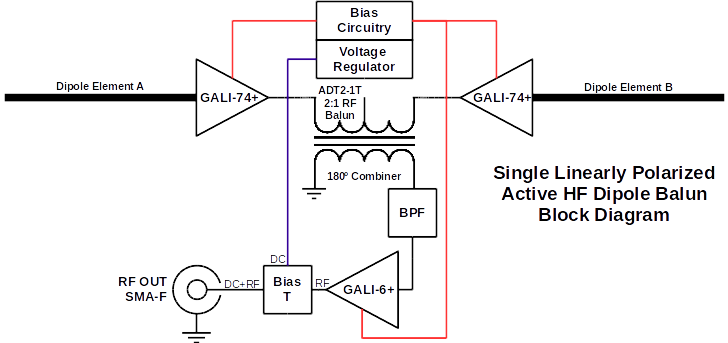
\includegraphics[width=0.75\linewidth]{figures/balun_block_diagram_2.png}
  \caption{Block Diagram of Single Polarization Active HF Dipole Balun.}
  \label{fig:block_diagram}
\end{figure}
